\section{Transformer}

The original Transformer model, introduced in the seminal 2017 paper Attention Is All You Need, marked a revolutionary shift in the field of NLP. 
\begin{figure}[H]
    \centering
    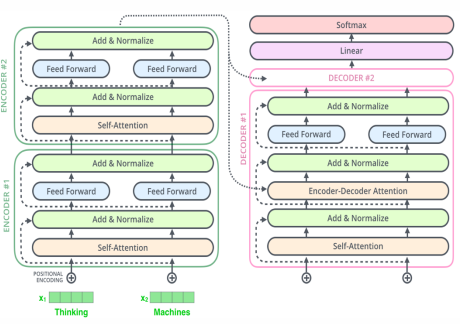
\includegraphics[width=0.5\linewidth]{images/nlp6.png}
    \caption{Transformer}
\end{figure}
At its core, the Transformer relies on a self-attention mechanism as its primary building block. 
This mechanism allows the model to dynamically focus on different parts of the input sequence when processing each token. 
The basic self-attention module consists of the following components:
\begin{enumerate}
    \item \textit{Multiple attention heads}: instead of relying on a single attention mechanism, the Transformer employs multiple attention heads that operate in parallel. 
        Each head computes attention independently, capturing different types of relationships between tokens. 
        These outputs are then concatenated and linearly transformed to produce the final result.
    \item \textit{Feed Forward Neural Network}: after the multi-head attention step, the output is passed through a Feed Forward neural network. 
        This network applies a non-linear transformation to the data, allowing the model to learn more complex patterns.
    \item \textit{Residual connections and layer normalization}: to facilitate training and improve gradient flow, the Transformer uses residual connections and layer normalization after each sub-layer. 
    \item \textit{Positional encoding}: this encoding provides information about the position of each token in the sequence, enabling the model to understand the sequential nature of language.
        Simplest way to do that would be to use a binary encoding of the position
        Since the embedding vector is made of floating point values, makes more sense to encode positions using sinusoids.
\end{enumerate}
\noindent The basic self-attention module is stacked multiple times to form the full Transformer architecture. This stacking allows the semantics of each token to build up progressively over multiple layers.
Each layer refines the representation of the input tokens by incorporating information from other parts of the sequence, resulting in rich, context-aware embeddings.

\paragraph*{Self-attention}
Self-attention is so valuable for language models. 
Words often have multiple meanings, and their interpretation depends heavily on the surrounding context.
Self-attention solves this problem by allowing a word's representation to adapt based on its context. 
It does this by learning a weighting function that prioritizes the most relevant parts of the input sequence when constructing a word's meaning. 
Essentially, it enables the model to focus on different words or phrases in the sentence, assigning more importance to those that matter most for understanding the current word.
This mechanism becomes even more powerful when stacked across multiple layers. 
With each layer, the model refines its understanding of relationships between words, enabling it to tackle complex linguistic tasks like co-reference resolution.

\subsection{Architecture}
The Transformer architecture is composed of three main components:
\begin{itemize}
    \item \textit{Input module}: this module generates the initial embedding for each token in the input sequence.
    \item \textit{Transformer blocks}: multiple transformer blocks are stacked on top of each other. Each block refines the embeddings by incorporating information from the surrounding context.
        Specifically, a transformer block modifies the embeddings through two key sub-components:
        \begin{enumerate}
            \item \textit{Self-attention block}: captures relationships between tokens by allowing each token to attend to others in the sequence.
            Contains multiple self-attention heads, each operating independently on a reduced embedding size of $\frac{d}{h}$, where $d$ is the original embedding dimension and $h$ is the number of attention heads.
            The self-attention mechanism relies on three key components:
            \begin{itemize}
                \item \textit{Query} ($Q$): represents the current token whose representation we are updating.
                \item \textit{Key} ($K$): encodes other tokens in the sequence, helping determine their relevance to the query.
                \item \textit{Value} ($V$): provides the actual content used to update the query's representation.
            \end{itemize}
            These components $(Q,K,V)$ are produced by applying linear transformations (matrices) to the original embeddings: 
            \[\text{attention}(Q,K,V)=\text{softmax}\left(\dfrac{QK^T}{\sqrt{d_k}}\right)V\]
            Here, $d_k=\frac{d}{\text{number of parallel attention heads}}$
            \item \textit{Feed-Forward Neural Network}: a simple, position-wise neural network that further processes the updated embeddings.
                Typically has a fan-out factor of 4, meaning the hidden layer is four times the size of the input embedding.
        \end{enumerate}
    \item \textit{Output module}: after the embeddings have been refined through multiple transformer blocks, this module decodes them to predict the next word or perform other downstream tasks.
\end{itemize}

\subsection{Transformer input}
Choosing between word-level and character-level representations involves balancing expressivity, sequence length, and the model's ability to generalize.
We have the following possibilities: 
\begin{itemize}
    \item \textit{Word-level tokens}: semantically rich and result in shorter sequences, reducing computational complexity. 
        However, they lead to larger vocabularies, struggle with out-of-vocabulary words, and ignore morphological details like prefixes or suffixes.
    \item \textit{Character-level tokens}: more flexible and capable of handling any word form, produce much longer sequences, increasing inference time.
        They also place the burden on the model to learn word structures from scratch, often leading to less interpretable embeddings.
    \item \textit{Sub-word tokens}: uses data-driven methods like Byte-Pair Encoding to identify frequent character sequences. 
    This approach captures common prefixes, suffixes, and word fragments, balancing vocabulary size and the model's ability to handle diverse linguistic patterns effectively.
\end{itemize}

\subsection{Bidirectional Encoder Representations from Transformers}
Bidirectional Encoder Representations from Transformers (BERT) revolutionizes text representation by learning deep contextualized embeddings through a masked language modeling approach.
During pre-training, BERT randomly masks words in the input using a special token and trains the model to predict these masked words.
This process helps BERT understand the relationships between words in a sentence, capturing rich linguistic patterns. 
Pre-trained on large corpora like Wikipedia and books, BERT provides powerful text representations without requiring manual feature engineering
The advantages of this model are: 
\begin{itemize}
    \item \textit{Eliminates feature engineering}: unlike traditional methods that rely on handcrafted features, BERT automatically learns meaningful representations.
    \item \textit{Preserves word order}: by leveraging bidirectional context, BERT retains word order and contextual relationships, outperforming count-based approaches.
    \item \textit{Unsupervised pre-training}: BERT benefits from unsupervised learning on vast amounts of text, enabling it to generalize well even with limited task-specific data.
\end{itemize}

\paragraph*{Fine tuning}
During pre-training, a special token is added at the start of every input sequence, but it is unused in the loss function. 
However, during fine-tuning, this token becomes crucial because the model is trained to produce a class label in place of the token.
Fine tuning works because BERT is pre-trained on massive datasets, it requires small data and has multilingual support. 

BERT can be used for text classification, sequence labelling and text pair classification and even question-answering tasks. 

\subsubsection{Document similarity}
BERT-based models can be effectively utilized to re-rank documents in web search tasks by predicting the relevance of documents to a given query.
This process involves fine-tuning the BERT model on a dataset of $\left\langle\text{query},\text{document}\right\rangle$ pairs, where the goal is to predict a relevance label for each pair.
To structure the input, the [SEP] token is used to separate the query and document, enabling the model to distinguish between the two components.

In addition to relevance prediction, BERT can also be fine-tuned to estimate semantic similarity between documents. 
This can be achieved through the following steps:
\begin{itemize}
    \item Start with a dataset consisting of pairs of similar documents and randomly selected pairs of (likely) dissimilar documents.
    \item Fine-tune a pairwise classifier to distinguish between similar and dissimilar document pairs.
    \item Use the logits or the predicted probability of the "similar" class as a measure of similarity between documents.
\end{itemize}
\noindent If ground truth similarity scores or distance metrics are available, the model can alternatively be fine-tuned for a regression task.
In this case, the objective is to directly predict the similarity score, providing a more precise measure of document similarity.

\subsubsection{Sentence transformer}
Using a pairwise BERT classifier to estimate the relevance of documents for a given query is highly effective due to BERT's ability to leverage the word order in both the query and the document and capture the semantics of words using contextual embeddings.
However, this approach is computationally expensive because BERT performs numerous matrix multiplications during inference.
It requires GPU acceleration to achieve reasonable speeds but still incurs significant latency.
A relevance score must be computed for every document in the collection, which becomes infeasible at scale.

To address these challenges, we aim to speed up computation by performing as much pre-computation as possible. 
However, since similarity scores depend on the query, precomputing them beforehand is not feasible. 
Below are two practical solutions:
\begin{enumerate}
    \item \textit{Lexical search with BERT re-ranking}: use a fast lexical search engine to quickly retrieve a candidate set of relevant documents.
        Apply the fine-tuned pairwise BERT classifier only to re-rank this smaller subset of candidates, significantly reducing computational overhead.
    \item \textit{Precompute document embeddings}: train BERT to generate embeddings for entire documents, compute similarity between documents using the dot product of their embeddings.
        Then, train the model on pairs of similar and dissimilar documents using a contrastive loss function, which gives high similarity scores for similar document pairs.
        Due to BERT's context length limitation , it may be necessary to split long documents into sections, compute embeddings for each section, and aggregate them.
\end{enumerate}
Sentence-BERT (SBERT) is a specialized framework that addresses these challenges by training BERT to learn fixed-length vector representations for entire sentences or documents.
It uses contrastive learning to create an embedding space where semantically similar documents produce similar embeddings.
In practice, SBERT trains two BERT models—one for encoding queries and another for encoding documents—and computes the similarity between them using the dot product (or cosine similarity) of their [CLS] token embeddings.
The model is trained on pairs of similar and dissimilar documents to ensure that similar documents yield high similarity scores and dissimilar documents yield low similarity scores.

\subsection{Generative Pre-trained Transformer}
Generative Pre-trained Transformer (GPT) is an auto regressive language model designed to predict the next token in a sequence. 
It achieves this by masking future tokens during training, ensuring the model only uses past and present context to make predictions.
This approach makes GPT particularly effective for text generation , as it learns to produce coherent and contextually relevant sequences by predicting one word at a time.
Unlike BERT, which uses bidirectional context, GPT predicts the next word based solely on preceding tokens, making it ideal for generating fluent and natural-sounding text.

\paragraph{Fine-tuning}
While GPT-2 can serve as a text encoder for classification tasks, its true strength lies in text generation. 
Therefore, it is particularly well-suited for tasks such as translation, summarization, dialogue generation, and more. 
During the fine-tuning process, specific strategies are employed to adapt the model effectively for these tasks. 

\subsubsection{Few shot learning}
Language models are highly versatile universal learners that can be utilized effectively with or without fine-tuning. 
During pre-training, these models are exposed to a vast number of examples of few-shot learning scenarios, enabling them to generalize and adapt to various tasks with minimal additional guidance. 
The ability to predict text serves as a flexible foundation for delivering a wide range of functionalities:
\begin{itemize}
    \item \textit{Translation}: even without explicit training for machine translation, models like GPT-2 have demonstrated the ability to perform translation tasks reasonably well. 
        For instance, despite being trained primarily on an English corpus, GPT-2 could translate between languages because some multilingual data was inadvertently included in its training set.
         While not the best-performing translation system, this showcases the model's inherent adaptability.
    \item \textit{Question Answering}: language models can store factual knowledge within their parameters and use it to answer questions. 
        For example, GPT-2 often provided accurate answers to questions, even though it was not explicitly trained for this task. 
        However, while confident predictions were usually correct, the reliability of such responses was not on par with dedicated question-answering systems at the time.
    \item \textit{Reading Comprehension}: by providing source context—such as a document containing relevant information—language models can extract answers and demonstrate reading comprehension. 
        This capability extends to tasks like fact-checking, where the model retrieves potential evidence supporting or refuting a claim by using the provided context.
    \item \textit{Summarization}: language models can generate concise summaries of longer texts, leveraging their understanding of context and relevance to distill key information effectively.
\end{itemize}